\chapter{The ICE Model}
Several terrestrial vertebrates, e.g. lizards, frogs, alligators and many birds, possess a hearing mechanism very different to
that of mammals: their tympanic membranes are coupled through large eustachian tubes and a large mouth cavity resulting in the influence of the vibrations of one tympanic membrane
on those of the other. This is illustrated in \ref{geckohead}. The typically small head sizes (compared to sound wavelength) of these animals result in
small phase differences (ITDs) and negligible amplitude difference (ILDs) between the ears. The coupling serves to enhance the ITDs and create ILDs
between the tympanal vibrations. These differences show directionality and serve as hearing cues for localization.

\begin{figure}[ht!]
 \centering
 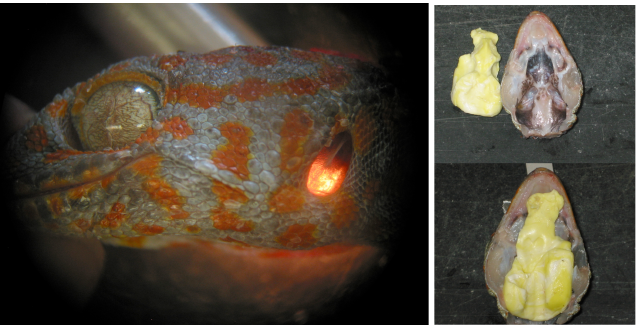
\includegraphics[width=.85\linewidth]{Diagrams/geckohead1.png}
 \caption[Illustration of a gecko's head]{Left: Picture of a Tokay gecko's head with the snout pointing to the left. The tympanic membrane is illuminated from behind by
 a light source on the other side of the head. The cartileginous extracolumella can be seen attached to the upper part of the membrane.
 Right: Cast imprint of the mouth cavity of the gecko with the snout pointing to the top. The figures illustrate the coupling of the tympani through the mouth cavity.
 Photographs courtesy of Jakob Christensen-Dalsgaard.}
  \label{geckohead}
\end{figure}

Proceeding from the earlier work done by Vossen in \cite{vossenthesis} and \cite{vossenjasa}, in this chapter we present a model for such a system of coupled ears with an emphasis on lizard hearing
- specifically the Tokay gecko and the common house gecko. Our goal is to demonstrate its main aspect of such a system - the coupling
of the eardrums through the mouth cavity. 
The main components of such a system are the mouth-cavity, the two tympani and the two \textit{extracolumella} (one on each tympanum). In general, the shape of the mouth-cavity is highly irregular and therefore
not conducive to an analytical treatment. Moreover, the system corresponds to a pair of coupled second-order PDE's with
moving boundaries. For this reason we will need to make further approximations in order to facilitate an
analytic solution.

In order to make the system more analytically tractable we will, as before, study a geometry in which a pair of rigidly clamped
linear elastic membranes are coupled through a cylindrical cavity. The cylindrical geometry allows an accurate calculation of the 
pressure distribution inside the cavity at both low and high frequencies. By accounting for the presence of the asymetrically attached
extracolumella, we will also explain the complex vibration patterns of the membrane. At the end of this chapter, we will
have the expressions that describe the steady-state vibrations of both eardrums as a function pressure amplitude, direction and frequency.

\section{Description of the Model}\label{description}
Before heading to a quantitative analysis of the ICE model, we will first need to list its basic components. 
and justify their properties based on a realistic mouth cavity. 

In Sec. \ref{subsecinnercavity}, we will describe the cylindrical model for the mouth cavity and state the reasons
for our choice of the geometry and the dimensions used. We will then proceed to describe the middle
ear system and its main components of interest, the \textit{extracolumella} and the \textit{tympani}
in Sec. \ref{middleear}. Finally, in Sec. \ref{soundinput} we will analyse the dependence of the acoustic input to both
eardrums on the direction of the sound source, head size and shape. 
\subsection{Mouth Cavity}\label{subsecinnercavity}
In the earlier treatment of the ICE model, the mouth canal is modelled as a simple cylinder closed at 
both ends by rigidly clamped (baffled) circular membranes; these model the tympanic membranes. As shown 
by Vossen in \cite[p.~21]{vossenthesis} and \cite{vossenjasa}, the length of the cylinder was chosen to be equal to the interaural distance and the radius of the model tympanum is
determined from the typical area of the realistic tympanum. The advantage of using a cylindrical cavity model for the mouth cavity is that the pressure
distribution inside the cavity is easy to calculate. The pressure distribution inside the cavity becomes highly non-uniform 
with increasing frequency and a cylindrical cavity simplifies its calculation. 

On the other hand, in this description the small area of the tympani results in a cavity volume which 
is an order of magnitude smaller than that of the realistic mouth-cavity in the corresponding animal. In general, a smaller volume results in a stronger coupling - both in terms of an increased iTD and an increased
iLD. For this reason, the earlier model overestimates the iTDs and iLDs at
low and high frequencies respectively.

In order to get around this problem we make some slight modifications to the model. Essentially, we maintain the cylindrical shape of the internal 
cavity but require it to have a volume which is equal to that of the realistic cavity ($V_{cav}$). We also maintain the same tympanum size and interaural distance
and can therefore calculate the radius of the cylinder as,
\begin{align}
 a_{cyl}=\sqrt{\frac{V_{cav}}{\pi L}}
\end{align}
\begin{figure}[ht!]
\begin{center}
\begin{subfigure}{1.0\textwidth}
 \centering
  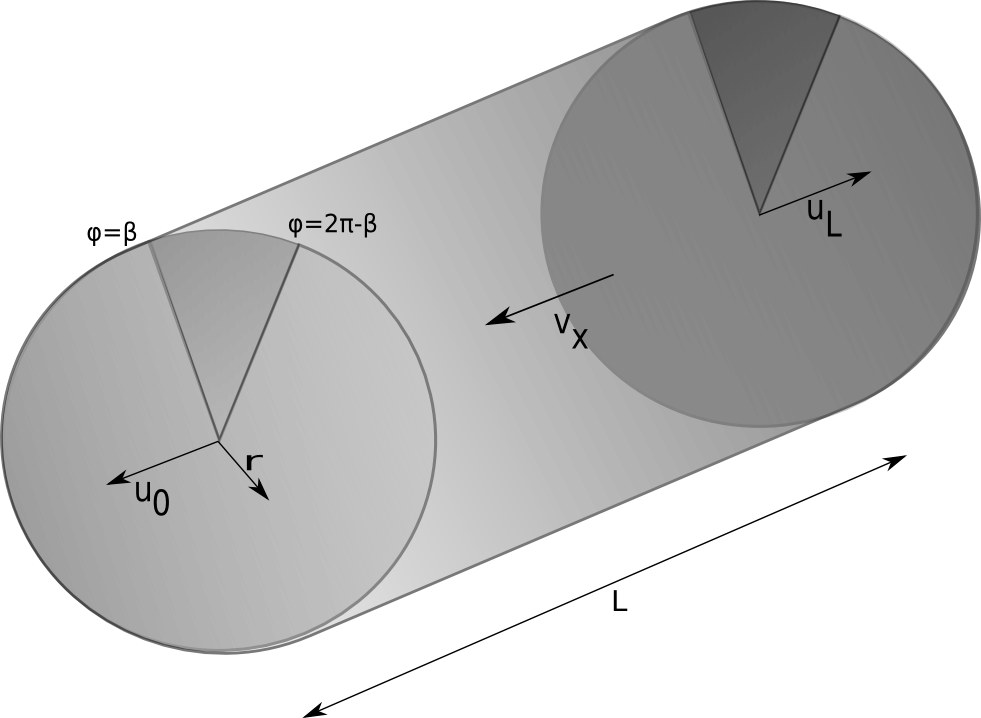
\includegraphics[width=.5\linewidth]{Diagrams/oldCylinder.png}
   \caption[Previous ICE Model Cylinder]{The previous geometric reprentation of the ICE model.}
  \label{oldICE}
\end{subfigure}

\begin{subfigure}{1.0\textwidth}
\centering
  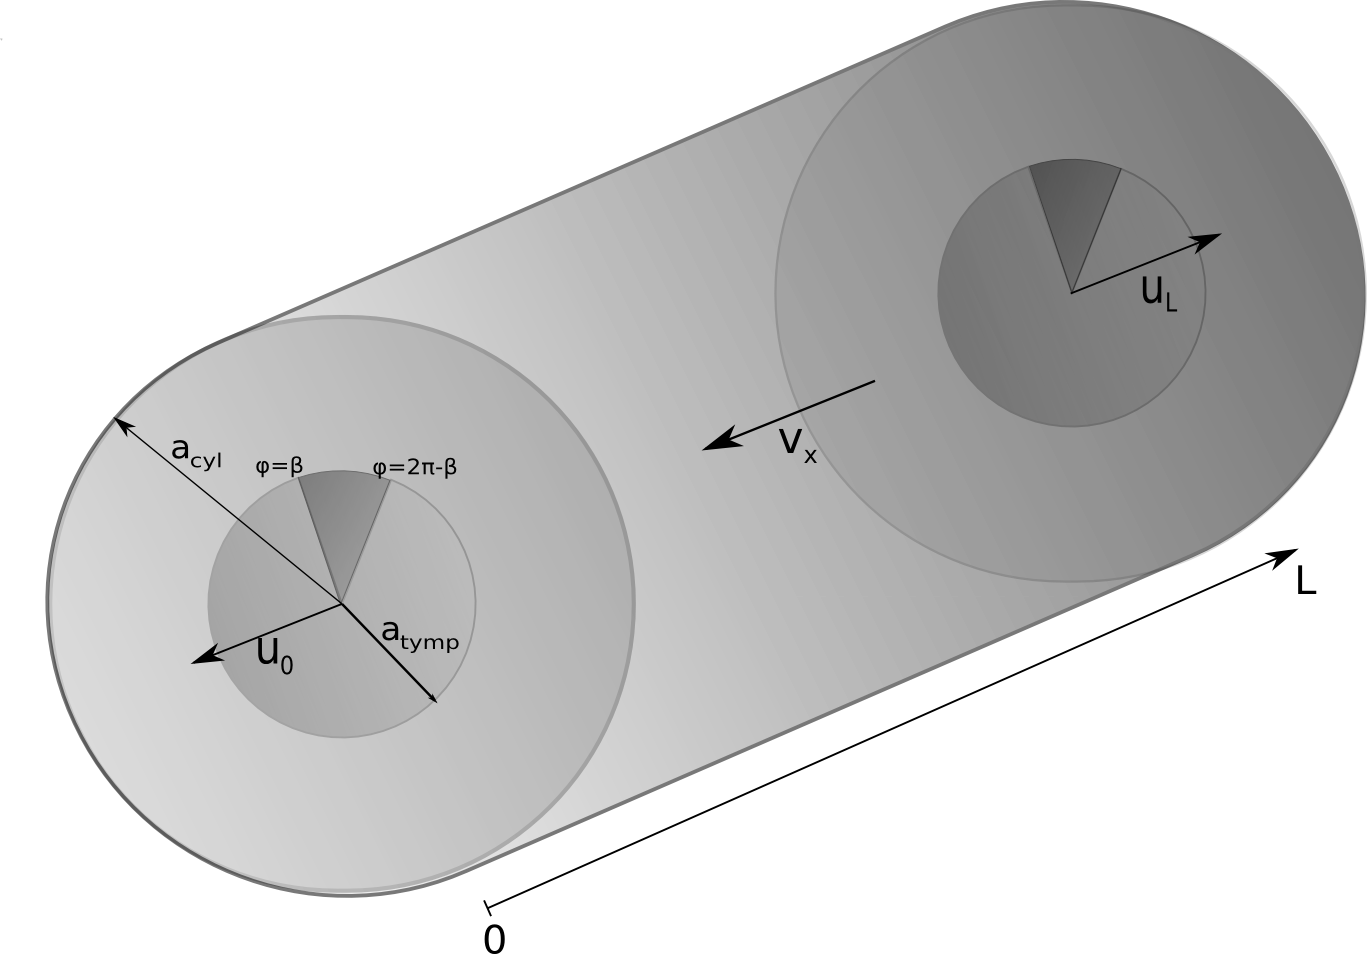
\includegraphics[width=.5\linewidth]{Diagrams/newCylinder.png}
  \caption[New ICE Model Cylinder]{The representation of the new model.}
  \label{newICE}
  \end{subfigure}
  \caption[Previous and current ICE model representations]{The bold arrows represent the direction conventions
  along the cylinder's axis. The new model is represented by a cylinder of radius $a_{cyl}$ and length $L$ closed
  at both ends by sectoral membrane of radius $a_{tymp}$.
  The darkly shaded region corresponds to the extracolumella (described in Sec. \ref{middleear}).}
\end{center}
\end{figure}
where $a_{cyl}$ is the cylinder radius and $L$ is the interaural distance. Simply put, the model consists of a cylindrical shell
of radius $a_{cyl}$ and length $L$ with circular holes on either side with the radius of the tympanic membrane, $a_{tymp}$. These
holes are in turn closed by rigidly clamped membranes which will be described in the next section. The previous and current geometric representations
of our model are shown in figures \ref{oldICE} and \ref{newICE}. The darkly shaded circular surfaces in fig. \ref{newICE} at ends $0$ and $L$ correspond to the two
eardrums.

We will be working with the cylindrical polar coordinates, $(r,\phi,x)$. The direction
along the cylindrical axis is denoted by $x$ and $(r,\phi)$ are the polar coordinates of the plane perpendular to the $x$-direction. 
Directions outward from the cylinder are taken as positive (in $x$) and those inward are taken as negative.
\subsection{Middle Ear System}\label{middleear}
The main components of the middle-ear of lizards are the two eardrums, the columella and the two cartileginous extracolumella.  
The tympanic membrane or the eardrum is a thin membrane that separates the outer ear and the
middle ear and vibrates in response to external sound waves.  Unlike humans, lizards 
possess only a single middle ear bone, the \textit{columella},
that is connected to both eardrums by means of a cartileginous element, the \textit{extracolumella}.

The membrane-extracolumella-columella system functions
as a second-order lever where the membrane - driven by the internal and external pressures - causes a displacement
of the extension of the extracolumella (known as the inferior process). This motion is in turn transmitted 
via the columella and columellar footplate to the inner ear (cochlea). The inner-ear translates this motion into
electrochemical impulses which will be passed on to the brain via the auditory nerve. The columella-extracolumella system effectively
transmits the mechanical vibrations from the eardrums to the inner ear. 
In the human middle-ear, the same function is
performed by the bones \textit{malleus, incus} and \textit{stapes}, which are collectively known
as the ossicles. 

For low frequencies (below $4$kHz), the extracolumella (or more accurately, the inferior process of the extracolumella)
moves as a completely stiff bar. It was shown by Manley \cite{manleygecko2} that the extracolumella begins to flex at higher frequencies - 
this is illustrated in fig. \ref{extracolumellaflection}. This is partly responsible for the poor high-frequency response of gecko middle ears - 
a feature also observed in other non-mammalian verterbates. The reason for this is that, due to the flection some energy is lost and
not transferred to the columella.

\begin{figure}[ht]
 \centering
 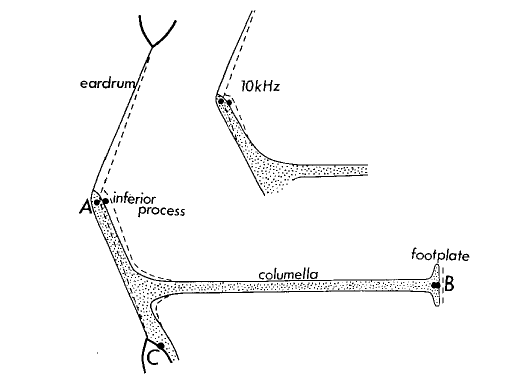
\includegraphics[width=.7\linewidth]{Diagrams/manleyextracolumellaflection.png}
 \caption[Extracolumella Flection]{Operation of the middle ear lever in geckos reproduced from \cite{manleygecko2}. The inferior process of the extracolumella (A-C) 
 hinges at point C at low frequencies. Also shown is the flection of the inferior process of the extracolumella.}
 \label{extracolumellaflection}
\end{figure}

\subsubsection{Tympanic Membrane}
The extracolumella applies a significant 
mechanical load on the tympanum and thereby precludes its treatment as a freely vibrating membrane. 
Furthermore, the contact surface of the malleus on the human eardrum is more or less symmetric whereas the 
extracolumella is attached asymetrically. This has important physical consequences - especially in the 
observed vibration patterns of the membrane.

In the previous treatment of the ICE model, the tympanum was modelled as a clamped circular membrane with assymetrically
attached sectoral load between $-\beta<\phi<\beta$ (\cite{vossenjasa}). This manifests itself as an additional
boundary condition at $\phi=\beta$ and $\phi=-\beta$ which has to satisfied via a numerical approximation. While
this method has the advantage of being able to accurately reproduce the complex vibration patterns of the eardrum, 
it does not lend itself well to an analytical treatment of the coupled system.

In our study, we will follow a slightly different path. The tympanic membrane will be modelled as a 
rigidly clamped sectoral membrane. This means that in addition to the radial boundary at $a_{tymp}$,
we have a new set of boundaries at $\phi=\beta$ and $\phi=2\pi-\beta$ where the membrane vibration is set to zero. This is illustrated in \ref{tympanummodel}.
The membrane material will be assumed to be linear-elastic. As before, the equations describing the vibrations of the membrane will 
consequently be linear $2^{nd}$-order PDE's.
\begin{figure}[ht]
 \centering
 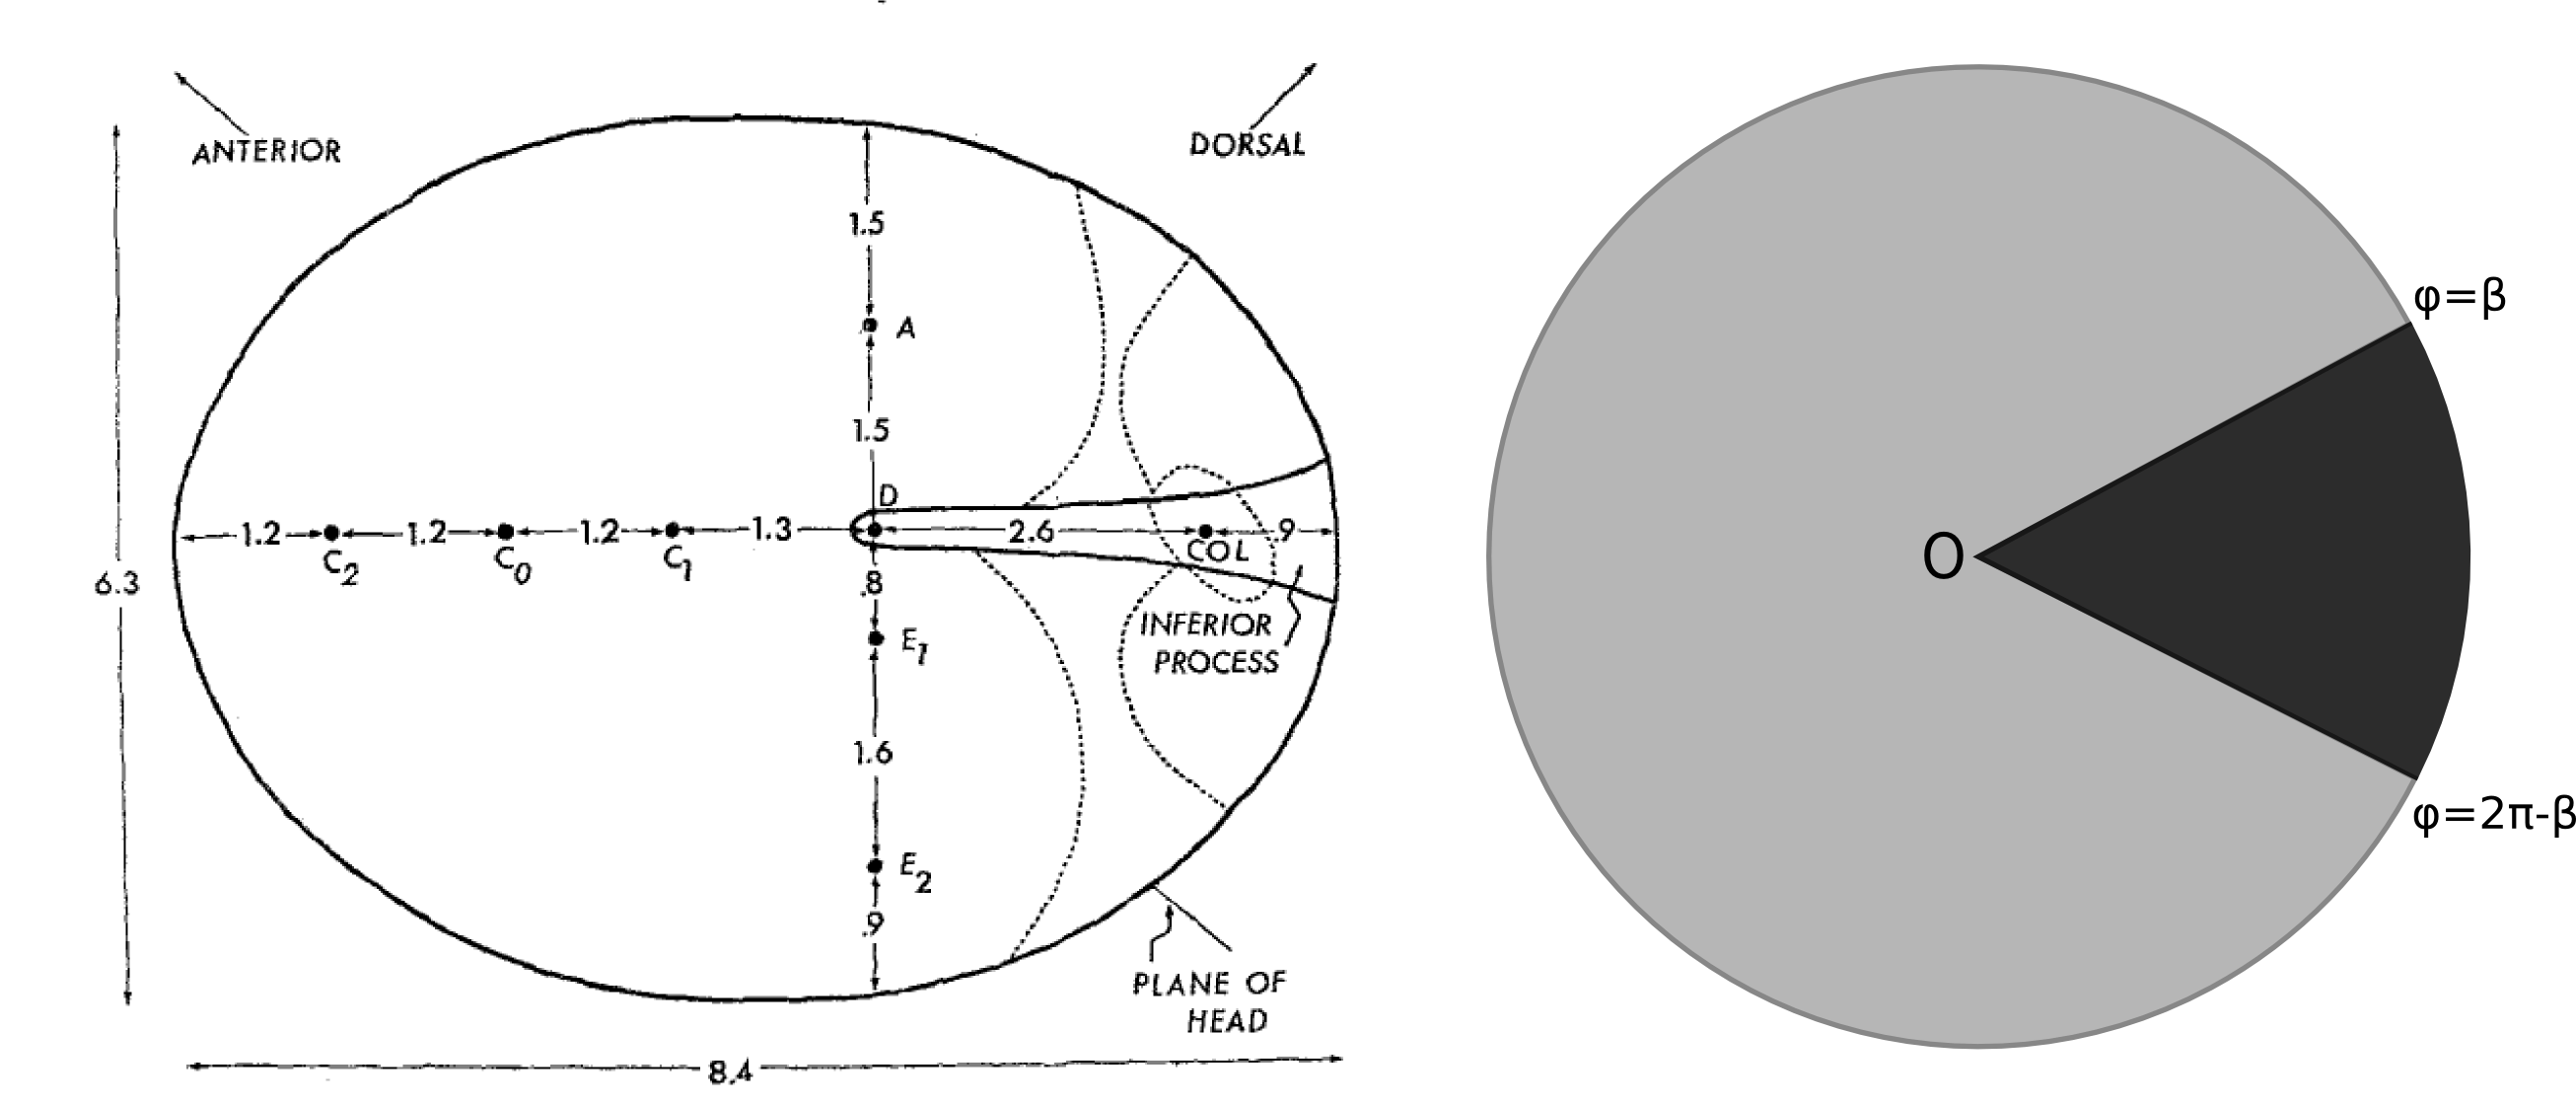
\includegraphics[width=.9\linewidth]{Diagrams/extracolumella2.png}
 \caption[Tympanic membrane model]{Left: Sketch of the eardrum of a Tokay gecko as seen from the outside taken from Manley, \cite{manleygecko1}. ``COL'' is
 the approximate position opposite the extracolumella insertion. The dots indicate the positions for measurements and will be discussed briefly in the
 next chapter. Dimensions
 in millimeters. Right: Our model for the loaded tympanic membrane. The lightly shaded region is modelled as a linear elastic membrane whereas the darkly shaded region 
 ($\beta<\phi<2\pi-\beta$) represents the contact surface of the extracolumella and the membrane. $\beta$ corresponds to the breadth of the extracolumella and is estimated from anatomical data.}
 \label{tympanummodel}
\end{figure}

At this point we should note that we have effectively set the mass of the extracolumella to infinity. Thereby, its motion has been neglected altogether. While this may seem counterintuitive at first, 
we will later see that this assumption, while simplifying the problem analytically,  has little effect on the physical phenomenon of interest, viz. the coupling between
the eardrums and the amplification of hearing cues. This will be discussed in-depth in Chapter \ref{modelanalysis}.

\subsection{Head Model and External Sound Input}\label{soundinput}
In realistic environments the acoustic fields experienced by animals are often very complex.
In addition to sound waves radiated directly from one or more sources in general, they also involve
waves reflected from objects in their immediate neighbourhood. Higher animals such as humans
possess the neural power to carry out the sophisticated signal processing needed to derive useful
information from these signals. Simpler animals like geckos respond to simpler cues - usually
the direct field from the nearest or strongest source.

We can therefore model our incoming wave as the simple case of an incident plane wave of a 
certain frequency. This input is specified in terms of its intensity, frequency and direction.
Such a stimulus can be generated in an anechoic chamber from loudspeakers which are placed at
a distance from the animal that is large compared to the animal's size and the wavelength
of the sound involved. Such experimental-setups are more thoroughly described by 
Christensen-Dalsgaard and Manley (\cite{dalsgaardmanley1}, \cite{dalsgaardmanley2}) and 
Christensen-Dalsgaard, Tang and Carr (\cite{dalsgaardtangcarr}).

The amplitude of the sound pressure incident on both ears can be taken as uniform in over 
the surface of the membrane. The spatial variation can be safely neglected because the
typical eardrum is less than $5$mm in diameter whereas the smallest sound wavelengths
in the hearing range of the larger lizards (eg. Tokay gecko) is around $70$mm ($4000$ Hz) 
and is around $50$mm ($7000$ Hz) for the smaller lizards (eg. Hemidactylus). In other
experiments, a similar stimulus has also been provided by means of a headphone sealed
to the ear (\cite{koepplcarr1}).

% In measuring the sound input, the important factors to be taken into account are
% \begin{itemize}
%  \item The separation of the ears and,
%  \item The overall head size
% \end{itemize}
In general a the sound on the other side of the head will differ in phase as well as amplitude. This is a result of the diffraction of 
sound around the head and body of the animal. The exact variation depends on the size of the animal and the frequency of the
incident wave. Due to the typically small head size of geckos, the amplitude variation 
(known as shadowing) is neglible (\cite{michelsenlarsen}). The phase difference, although small compared to those in larger animals, 
cannot be neglected. We can therefore consider the sound wave with angular frequency $\omega$ to have a constant (pressure) amplitude $p$
on the head.

In the earlier ICE model, the effect of diffraction on the phase difference was neglected as well. The phase difference
is found directly from the phase difference $\Delta$ as shown in fig. \ref{fig:oldheadmodel}.
As a result, the sound pressure inputs at both ears is given by,
\begin{equation}\label{oldsoundinput}
p_0=pe^{j\omega t} e^{-k\Delta/2},\qquad p_L=pe^{j\omega t} e^{k\Delta/2},\qquad \Delta=L\sin\theta.
\end{equation}
We note that in defining the input in this way, we've emphasized the symmetry of the system.
The ear closer to the sound source is referred to as the \textit{ipsilateral} ear and
is denoted by a subscript $0$ and the one further away from the source is referred to as the \textit{contralateral} ear and is denoted by a subscript $L$. 
Subsequently, unless otherwise specified, the subscripts $0$ and $L$ will correspond to the ipsi- and contralateral ears respectively.
\begin{figure}[ht]
 %\centering
 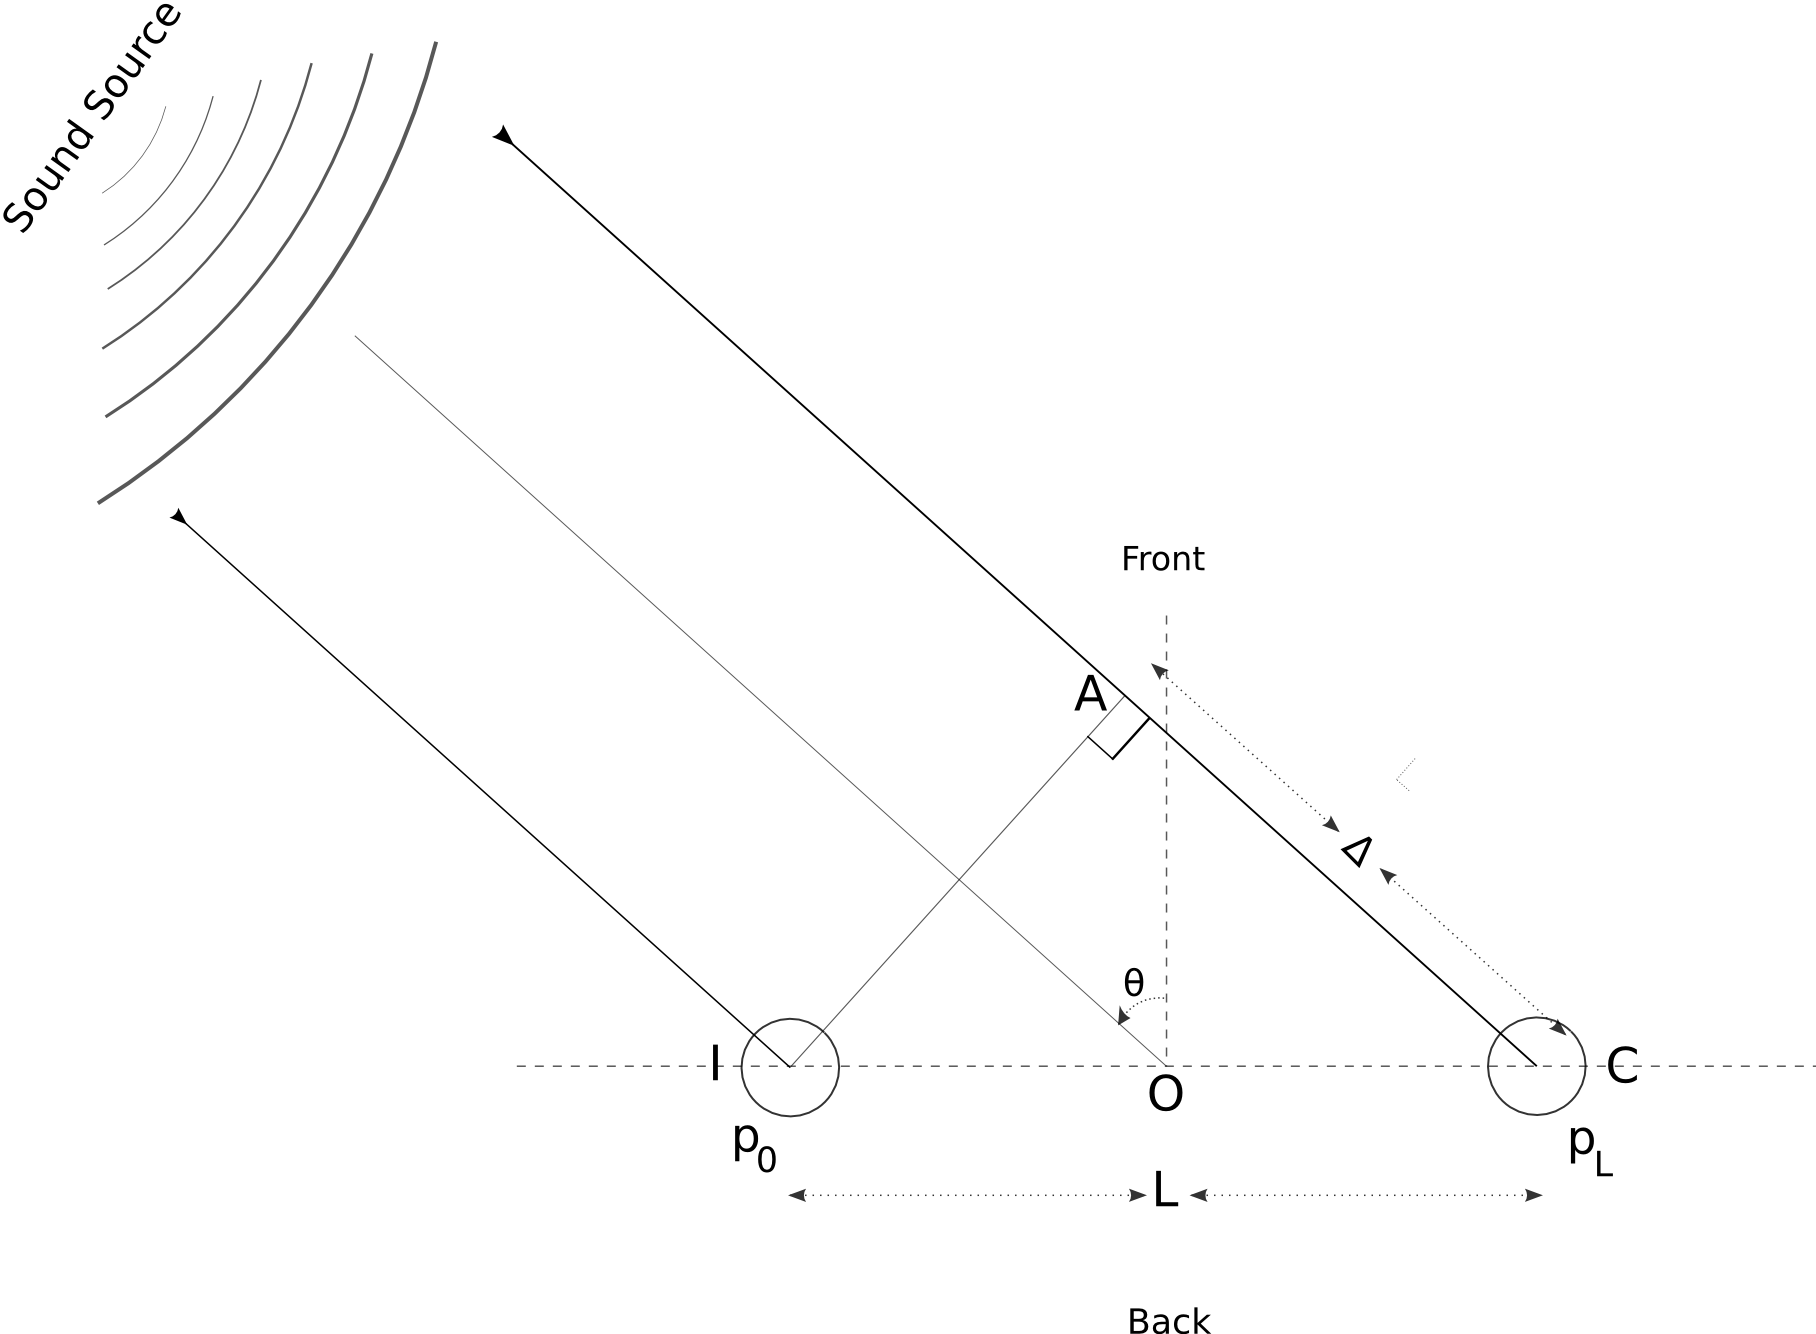
\includegraphics[width=.75\linewidth]{Diagrams/acousticheadmodelold.png}
 \caption[Previous acoustic head model for geckos]{The previous acoustic head model for geckos. The extra distance travelled by the sound wave to reach the contralateral ear 
 is denoted by $\Delta$.}
 \label{fig:oldheadmodel}
\end{figure}
We have also chosen a coordinate
system relative to the \textit{median-sagittal} plane or the head midline of the animal and $\theta$ gives the angle of incidence of this
sound wave relative to this plane. For more complex auditory systems we would require two angles $(\theta, \phi)$ to describe
the three-dimensional system but in our analysis this is unnecessary. For the animals we are concerned with, i.e. geckos, the natural
predators and prey are usually present on the same plane as the animal and our assumption is therefore reasonable.

\begin{figure}[ht]
 %\centering
 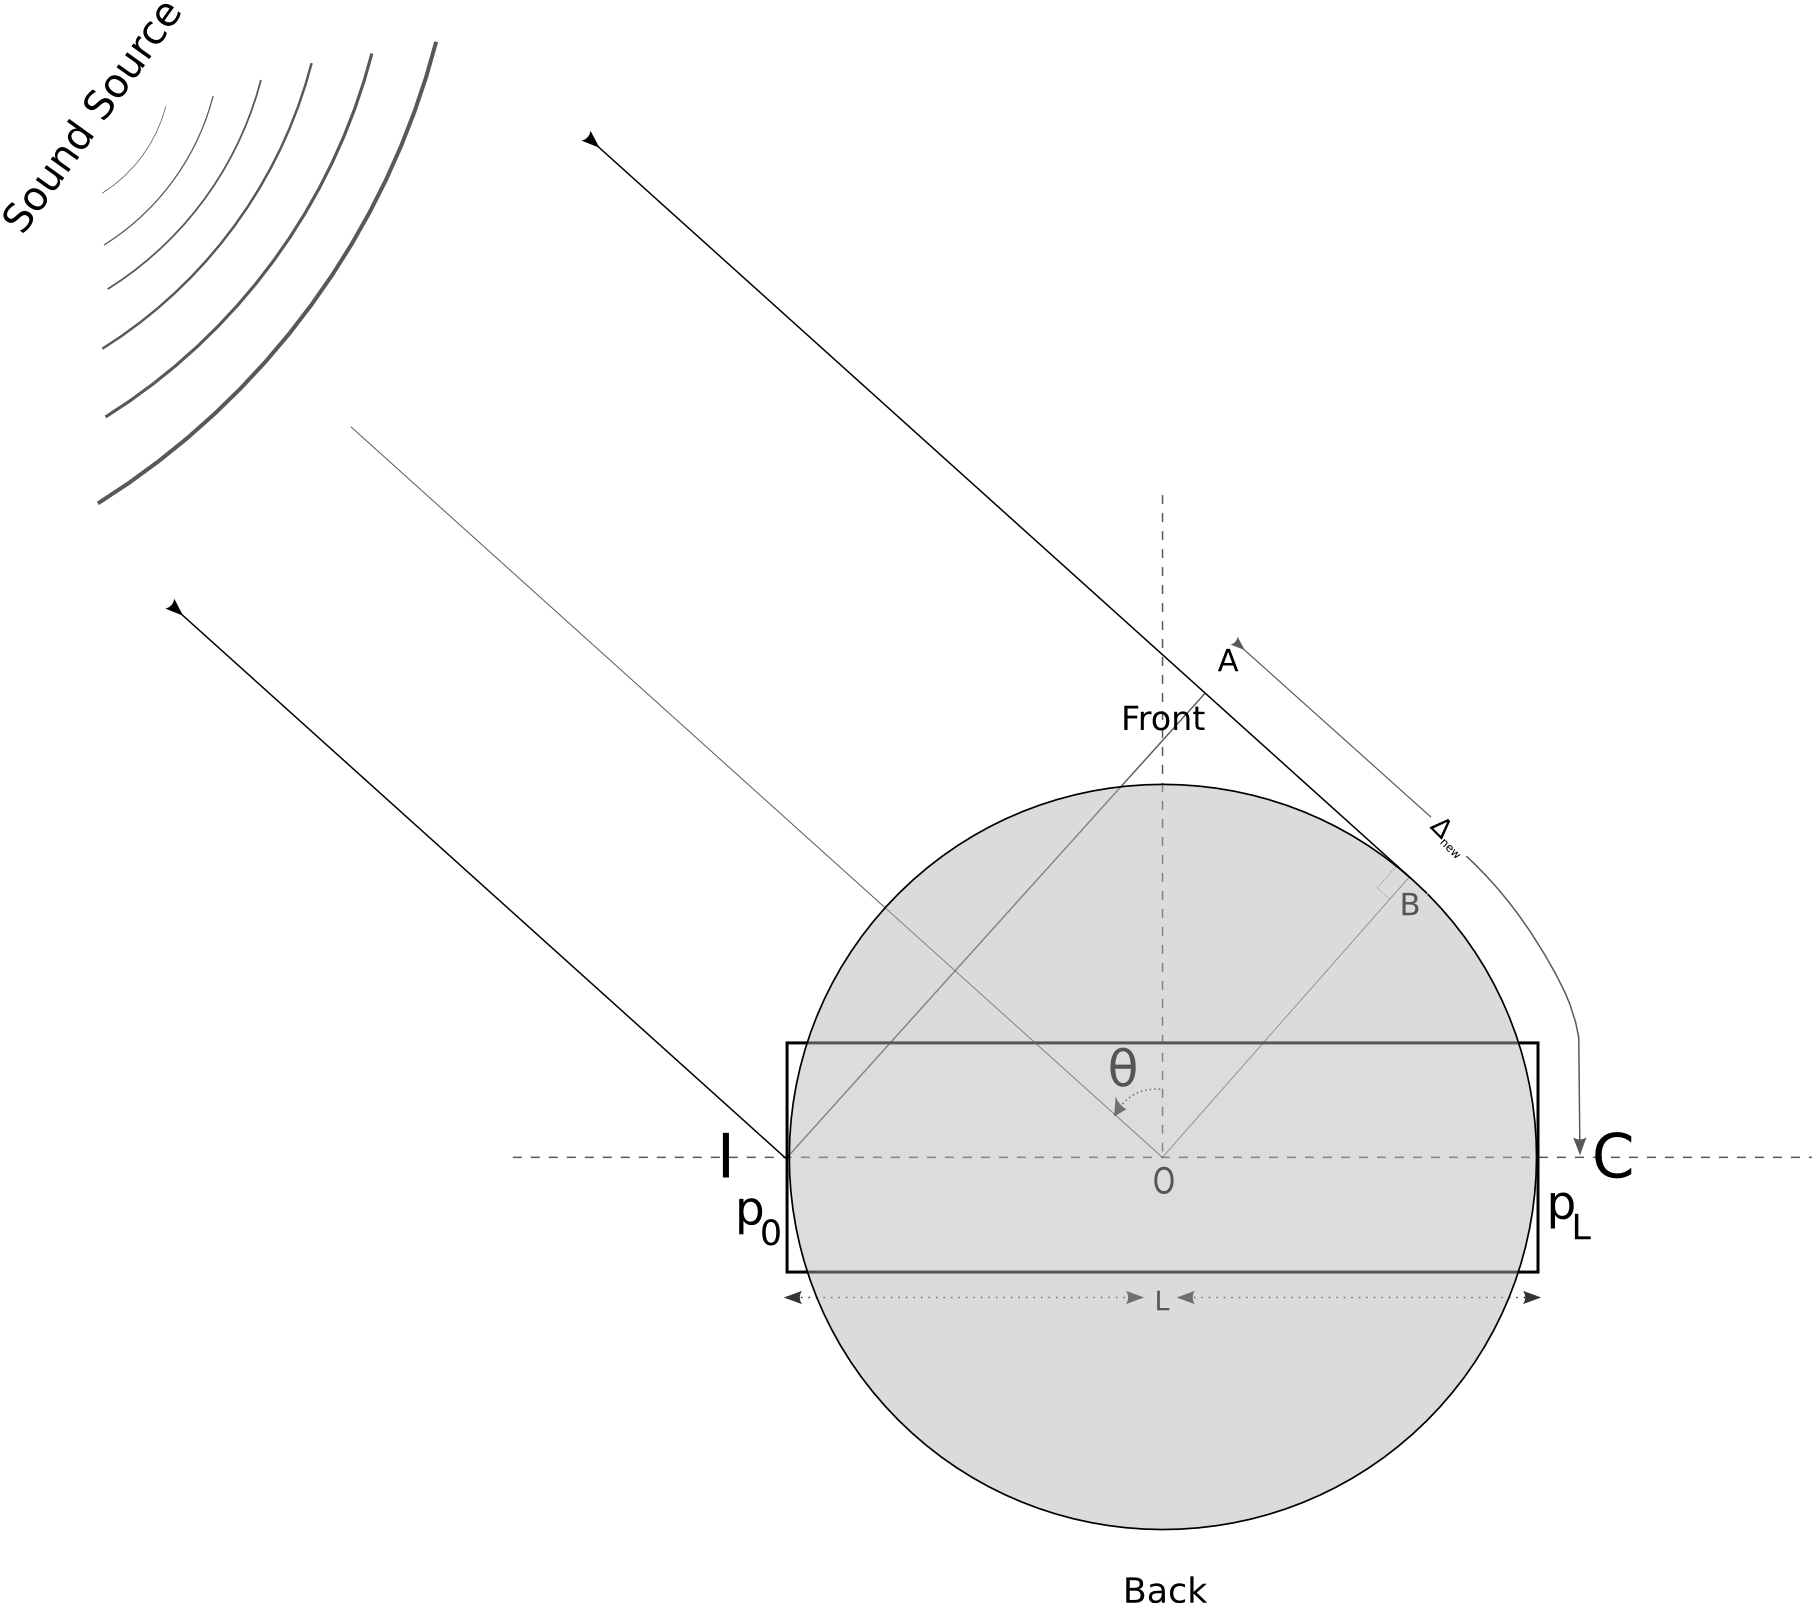
\includegraphics[width=.75\linewidth]{Diagrams/acousticheadmodel2.png}
 \caption[New acoustic head model for geckos]{The acoustic head model for geckos. The rectangular outline 
 is the internal cavity. As before, the extra distance travelled by the sound wave to reach the contralateral ear is given by 
 $\Delta$. In this case, however, we have accounted for the influence of diffraction around the head on the phase difference between the inputs
 to both ears.}
 \label{newheadmodel}
\end{figure}
In our model we model the head as a sphere with a diameter equal to the interaural separation. As a result the sound has to travel around the 
head in order to reach the contralateral ear resulting in a longer path. The frequency domain solution for the diffraction of sound around a
sphere was obtained by Lord Rayleigh at the end of the $19^{\mbox{th}}$ century (\cite{rayleigh1},\cite{rayleigh2}). The expressions 
are greatly simplified at low frequencies and the phase difference is simply increased by by a factor of $1.5$ (i.e. $\Delta_{new}=1.5\Delta$). The new model is illustrated in Fig. \ref{newheadmodel}.
\section{Derivation of the Model}
We will now use the previously described physical model to derive the main expressions of interest in the ICE model - the membrane
vibration profiles, the ipsi- and contraleteral filters and the cavity pressure distribution. We will thus find an expression for the pressure 
distribution in the cylindrical cavity and for the membrane vibrations subject to an external stimulus. After applying the 
appropriate boundary conditions to relate the membrane vibrations to the internal pressure, we will find the expression for the membrane
vibrations as a function of direction and frequency.

We will start in Sec. \ref{internalcavity} by finding a general solution to a $2^{nd}$-order PDE - the $3$D wave
equation - that describes the pressure distribution inside the cylindrical cavity. In this section we will introduce the
main boundary condition the pressure will be subject to - the ``no-penetration'' boundary condition. This is a physical requirement that results from the fact that the air
inside the cavity does not penetrate a solid boundary.

In Sec. \ref{membranevibrations} we will solve for the vibrations of the tympanic membranes. As an example, we
will find an expression for the free and periodically driven vibrations of a circular membrane. Using the methods
developed in this section, we will solve for the vibrations of a sectoral membrane - which, as we have already discussed,
models the loaded tympanum. The final expression will correspond to the steady-state vibrations of a linear elastic
membrane. As we neglect the transient response of the membrane, we will also discuss the circumstances under which this
is justified.

In Sec. \ref{coupledmembranes} we will conclude by using our knowledge to solve for the vibration of the fully coupled
system. In this section we will  proceed by applying the velocity boundary condition at either end of the cylinder. In
order to help with our analysis, we will present a simplification scheme for this boundary condition. We will end this section
by defining the ipsi- and contralateral filters. The final expressions that give us the vibrations 
of the tympanic membranes as a function of the external pressure with the influence of the internal cavity encoded in the ipsi- and contralateral filters. 
We have listed the main parameters and functions used in our analysis (including the geometry parameters) in Tables \ref{parametertable}
and \ref{functiontable}.

\begin{minipage}{\linewidth}
\renewcommand{\arraystretch}{1.2}
%\caption{Parameters and Functions used in the ICE Model} \label{parametertable} 
\centering
\captionof{table}{Functions and Parameters used in the ICE Model} \label{parametertable} 
\begin{tabular}{c p{12 cm}}
\hline
$\theta$ & Direction of the sound source with respect to the head midline.\\
$\omega$ & Angular frequency of the incoming sound wave.\\
$k$ & Wavenumber $k=\omega/c$ with $c=343$m/s being the speed of sound.\\
$p$ & Pressure amplitude of the incoming sound wave.\\
$\Delta$ & Phase difference between the sound wave reaching the contra- and ipsilateral ear.\\
$p_{0/L}$ & Sound pressure on the ipsi- ($x=0$) and contralateral ($x=L$) ears respectively.\\
%& \\
$(x,r,\phi)$ & Cylindrical polar coordinates with $x$ being the axial direction.\\
$L$ & Interaural separation and length of cylinder.\\
$a_{cyl}$ & Radius of cylinder.\\
$a_{tymp}$ & Radius of tympanum.\\
$\beta<\phi<2\pi-\beta$ & Extent of the vibrating part of the membrane. The rest of the circle corresponds to
the extracolumellar footplate.\\
$V_0$ & Volume of the cavity.\\
\hline
\end {tabular}\par
\bigskip
\end{minipage}

\begin{minipage}{\linewidth}
\renewcommand{\arraystretch}{1.2}
%\caption{Parameters and Functions used in the ICE Model} \label{parametertable} 
\centering
\captionof{table}{Functions and Parameters used in the ICE Model contd.} \label{functiontable} 
\begin{tabular}{c p{12 cm}}
\hline
$J_q$ & Order $q$ Bessel function of the first kind.\\
$\mu_{qs},\nu_{qs}$ & Respectively - $s^{th}$ zero and $s^{th}$ extremum of the above Bessel function.\\
$f_{qs}(x,r,\phi)$ & Orthogonal modes for the pressure distribution inside the mouth cavity.\\
$\zeta_{qs}$ & Wavenumber of the above modes in the $x$-direction.\\
$p(x,r,\phi;t)$ & Pressure distribution inside the mouth cavity.\\
$v_x(x,r,\phi;t)$ & Velocity function inside the mouth cavity.\\
&\\
$u_{mn}(r,\phi;t)$ & Eigenmodes of the membrane displacement function.\\
$\omega_{mn}$ & Eigenfrequency of the above eigenmodes.\\
$Q$ & Quality factor of the membrane.\\
$\Psi(r,\phi;t)$ & Driving pressure on the membrane.\\
$u_{0/L}(r,\phi;t)$ & Membrane displacement function.\\
$S^{0/L}(t)$ & Total membrane displacement.\\
&\\
$G_{ipsi}(r,\phi)$ & Ipsilateral filter.\\
$G_{contra}(r,\phi)$ & Contralateral filter.\\
\hline
\end {tabular}\par
\bigskip
\end{minipage}
\subsection{Internal Cavity}\label{internalcavity}
We assume that the air inside the cavity obeys linear acoustics (cf. acoustic textbooks such as \cite[p.~313]{rschevkinsound} and \cite[p.~247]{temkinelements} ). 
This means that the air moves due to pressure $p(x,r,\phi;t)$ whose distribution inside the cavity
is given by the $3$D acoustic wave-equation in cylindrical polar coordinates,	
\begin{equation}\label{pressurewaveeqn}
 \frac{1}{c^2}\frac{\partial^2 p(x,r,\phi,t)}{\partial t^2}=\frac{1}{r}\frac{\partial}{\partial r}\left(r\frac{\partial p(x,r,\phi,t)}{\partial r}\right)
 +\frac{1}{r^2}\frac{\partial p(x,r,\phi,t)}{\partial \phi^2}+\frac{\partial p(x,r,\phi,t)}{\partial x^2}
\end{equation}
where $c$ is the sound propagation velocity. The complete solution must take into account the boundary conditions at and within the cavity walls and the
ones at the air-membrane interface. We also note that the above equation implies that the animal's mouth is closed, which is typical for a waiting
animal. In order to solve \eqref{pressurewaveeqn} for a particular frequency $f$ (angular frequency $\omega=2\pi f$), we use the following
separation ansatz
\begin{equation}\label{pseparationansatz}
  p(x,r,\phi,t)=f(x)g(r)h(\phi)e^{j\omega t}
\end{equation}
which after substitution into the acoustic wave-equation leads to,
\begin{equation}\label{pseparationansatz2}
\begin{split}
 k^2f(x)g(r)h(\phi)+&f(x)h(\phi)\left[\frac{\partial^2 g(r)}{\partial r^2} + \frac{1}{r}\frac{\partial g(r)}{\partial r}\right] \\
 &+f(x)g(r)\frac{1}{r^2}\frac{\partial h(\phi)}{\partial \phi}+\frac{\partial^2 f(x)}{\partial x^2}=0
\end{split}
\end{equation}
with $k:=\omega/c$. This results in the following set of separated ODE's,
\begin{align}
 \frac{d^2 f(x)}{dx^2}+\zeta^2f(x)&=0\\
 \frac{d^2 h(\phi)}{d\phi^2}+q^2h(\phi	)&=0\\
 \frac{\partial^2 g(r)}{\partial r^2} + \frac{1}{r}\frac{\partial g(r)}{\partial r}+\left[(\displaystyle\underbrace{k^2-\zeta^2}_{=:\nu^2})-\frac{q^2}{r^2}\right]g(r)&=0\label{besselequation1}
\end{align}
with separation constants $q$ and $\zeta$. The last equation is the Bessel differential equation \cite[p.~313]{copsonbessel} and its general solution is given by,
\begin{equation}
 g(r)=C_{qs}J_q(\nu r)+D_{qs}Y_q(\nu r).
\end{equation}
$J_q$ and $Y_q$ are the order-$q$ Bessel functions of the first and second kind respectively. The Bessel function of the second kind can be ignored as it diverges at $r=0$.
The solutions to the separated equations are therefore given by,
\begin{equation}
 f(x)=e^{\pm \zeta x},\ h(\phi)=e^{\pm j\phi},\text{and}\ g(r)=J_q(\nu r)
\end{equation}
with a specific solution to \eqref{pressurewaveeqn} given by,
\begin{equation}\label{specificpressure1}
 p(x,r,\phi;t)=\left[(A^+e^{jq\phi}+A^-e^{-jq\phi})e^{j\zeta x}+(B^+e^{jq\phi}+B^-e^{-jq\phi})e^{-j\zeta x}\right]J_q(\nu r)e^{j\omega t}.
\end{equation}
The coefficients $A^\pm$, $B^\pm$, $q$, $\zeta$ and $\nu$ will be subsequently determined by the boundary conditions. 

In general, the time component of the pressure also has a \textit{backward-moving} component, i.e. $e^{-j\omega t}$. By making the ansatz in \eqref{pseparationansatz}, 
we have implicitly made use of the fact that the form of the input constrains the pressure to only have a \textit{forward-moving} component, i.e. $e^{j\omega t}$.  
\subsubsection{Pressure Boundary Conditions}\label{pressureboundaryconditions}
There are three sets of boundary conditions - 
\begin{itemize}
 \item Continuity and smoothness in $\phi$ which is equivalent to $h(0)=h(2\pi)$ and $h^\prime(0)=h^\prime(2\pi)$ where, $h^\prime=dh/d\phi$.
 \item Vanishing of the normal derivative at the cavity walls - $g^\prime(a_C)=0$ ($a_C$ is the radius of the cylinder).
 \item Equating the membrane velocity to the velocity function at the membrane boundaries (to be discussed in the next section).
\end{itemize}
The first set of requirements is obvious. This reduces \eqref{specificpressure1} to 
\begin{equation}\label{specificpressure2}
 p(x,r,\phi;t)=\left[Ae^{j\zeta x}+Be^{-j\zeta x}\right]\cos q\phi J_q(\nu r)e^{j\omega t}.
\end{equation}
With $q$ constrained to be an integer.

The second and third are a result of the so called ``no-penetration'' boundary-condition
of fluid-mechanics. It arises from the from the fact that the cavity wall is an impermeable boundary. This translates 
into the requirement that the normal velocity function should vanish (\cite[p.~111]{pozrikidisFluid}).
The velocity function ($\mathbf{v}$) is related to the pressure by, 
\begin{equation}\label{pressurevelocityrelation}
 -\rho\frac{\partial \mathbf{v}}{\partial t}=\nabla p
\end{equation}
At the cylindrical cavity wall, the normal velocity is in the radial direction.
Substituting the expression for pressure in \eqref{specificpressure1} in the above equation leads to
a Neumann boundary condition for the pressure,
\begin{align}\label{radialnopenetration}
 v_r=-\left.\frac{1}{j\rho\omega}\frac{\partial p(x,r,\phi;t)}{\partial r}\right\vert_{r=a_C}&=0\nonumber\\
    \Rightarrow\left.\frac{\partial J_q (\nu r)}{\partial r}\right\vert_{r=a_C}&=0
\end{align}
This constrains $\nu$ to a discrete set of values which correspond to the local minima and maxima
of $J_q$. We can therefore index $\nu$ by $q$ and $s=0,1,2,3,\ldots$ with $\nu_{qs}=z_{qs}/a_C$:
$z_{qs}$ being the $s^{th}$ extremum of the order-$q$ Bessel function of the first kind.
This results in a discrete set of modes that satisfy \eqref{pressurewaveeqn} which are given
by,
\begin{equation}\label{specificpressure3}
 p_{qs}(x,r,\phi;t)=\left[A_{qs}e^{j\zeta_{qs}x}+B_q{s}e^{-j\zeta_{qs}x}\right]f_{qs}(r,\phi)e^{j\omega t}
\end{equation}
where we have added the subscripts $q$ and $s$ to $\zeta$ and denoted the $(r,\phi)$ part of \eqref{specificpressure2}
by $f_{qs}(r,\phi)$. Effectively, the
modes are 3D waves propagating with wave numbers $\zeta_{qs}$ in the $x$-direction and $\nu_{qs}$ in the radial
direction. The first of these modes (corresponding to $q=0,s=0$) is of particular importance. Since the first
maximum of $J_0$ occurs at $r=0$, we have $\nu_{00}=0$. This leads to the first mode being a plane-wave which
is constant in $r$ and $\phi$ and only varies in $x$. 

A very useful property of the above modes is their orthgonality, i.e.
\begin{equation}\label{pressureorthogonality}
 \int_\Omega dVp_{q_1s_1}p_{q_2s_2}=0,\ if\ q_1\neq q_2\ or\ s_1\neq s_2
\end{equation}
the integral is over the volume	 of the cylinder. This is a consequence of the fact that for different $q$'s
the cosine parts of the modes are orthogonal whereas for a given $q$ the Bessel parts are orthogonal for
different $s$'s or expressed as an equation,
\begin{equation}\label{besselorthogonality}
 \int dS f_{q_1s_1}f_{q_2s_2}=0,\ q_1\neq q_2\ or\ s_1\neq s_2
\end{equation}
where $dS=rdrd\phi$ and the integral being taken over the disk of radius $a_C$.
We can therefore write the general solution to \eqref{pressurewaveeqn} as a linear combination of the orthogonal modes given in \eqref{specificpressure3},
\begin{equation}\label{pressuregeneral1}
 p(x,r,\phi;t)=\displaystyle\sum^\infty_{q=0}\displaystyle\sum^\infty_{s=0}\left(A_{qs}e^{j\zeta_{qs}x}+B_{qs}e^{-j\zeta_{qs}x}\right)f_{qs}(r,\phi)e^{j\omega t}
\end{equation}
The remaining coefficients, $A_{qs}$ and $B_{qs}$, will be determined by equating the velocity function to
the membrane velocity at both ends of the cylinder. To do so, we will first need to find an expression
for the membrane vibrations - as we will in the following section.

\subsection{Vibration of the Membrane}\label{membranevibrations}
As a preliminary exercise, we will first derive expressions for the free and force-driven
vibrations of a circular membrane. We will then use our results to move on to the sectoral membrane 
which corresponds to the tympanum loaded by the extracolumella. Thi corresponds to the approximating
the extracolumella to have infinite mass. 
\subsubsection{Circular Membrane}
The equation of motion for the vibration of a rigidly clamped circular membrane of radius $a_M$ solves for the membrane displacement $u$ at
a point $(r,\phi)$ with $r<a$ and $0<\phi<2\pi$. It is given by,
\begin{equation}\label{membraneequation1}
 \begin{split}
 -\frac{\partial^2 u(r,\phi;t)}{\partial t^2}-2\alpha\frac{\partial u(r,\phi;t)}{\partial t}+c^2_M \left[\frac{1}{r}\frac{\partial}{\partial r}\left(r\frac{\partial u(r,\phi,t)}{\partial r}\right)\right. +\frac{1}{r^2}&\left.\frac{\partial u(r,\phi,t)}{\partial \phi^2}\right]
 \\ &=\frac{1}{\rho_M d}\Psi(r,\phi;t)
 \end{split}
\end{equation}
subject to the boundary condition $u(r,\phi;t)|_{r=a_M}=0$.. We've defined the following membrane material properties,
\begin{itemize}
 \item $c_M$ - propagation speed of vibrations.
 \item $\alpha (>0)$ - the damping coefficient.
 \item $\rho_M$ - density.
 \item $d$ - thickness.
\end{itemize}
$\Psi(r,\phi;t)$ is the pressure on the membrane surface at $(r,\phi)$. In our discussion we are only concerned with periodic and uniform 
pressure acting on the membrane surface. As we have already stated in Sec. \ref{soundinput},  the small size of the membrane with respect to the sound wavelength,
justifies the spatial uniformity of our input.
\subsubsection*{Free Vibrations}
\noindent\textbf{Undamped Membrane}: We first determine the eigenmodes of an undamped circular membrane by solving \eqref{membraneequation1} for $\alpha=0,\ \Psi=0$
(the resultant equation is better known as the $2$D Helmholtz equation, cf. \cite[p.~187]{asmar2005partial}). Just as we did in \eqref{pseparationansatz},
we do this by making a separation ansatz ,
\begin{equation}\label{mseparationansatz}
 u(r,\phi;t)=f(r)g(\phi)h(t)
\end{equation}
This gives us the following set of equations
\begin{align}
 \frac{\partial^2 f(r)}{\partial r^2} + \frac{1}{r}\frac{\partial f(r)}{\partial r}+\left[\mu^2-\frac{m^2}{r^2}\right]f(r)&=0\label{besselequation2}\\
  \frac{d^2 g(\phi)}{d\phi^2}+m^2g(\phi)&=0\\
 \frac{d^2 h(t)}{dt^2}+c^2_M\mu^2h(t)&=0
\end{align}
with separation constants $\mu$ and $m$. The solution of the first of these equations should already be familiar to us from the previous section - $J_m(\mu r)$,
 the order-$m$ Bessel function of the first kind. The boundary conditions in $\phi$ direction remain the same resulting in,
\begin{equation}\label{specificmembrane1}
 u(r,\phi;t)=\left[(M^+e^{jm\phi}+M^-e^{-jm\phi}\right)e^{jc_M\mu t}+(N^+e^{jm\phi}+N^-e^{-jm\phi})e^{-jc_M\mu t}] J_m(\mu r)
\end{equation}
Unlike in the case of the internal cavity, we require $u$ to vanish at the boundary so we have a Dirichlet boundary condition which
effectively requires: $J_m(\mu a_M)=0$. This constrains $\mu$ to a discrete set of values which correspond to the zeros of $J_m$. The eigenmodes of a 
the circular membrane are therefore given by,
\begin{equation}\label{membraneeigen}
\begin{split}
 u_{mn}(r,\phi;t)=\left[(M^+_{mn}e^{jm\phi}+M^-_{mn}e^{-jm\phi})\right.& e^{j\omega_{mn} t}+ \\
 &\left.(N^+_{mn}e^{jm\phi}+N^-_{mn}e^{-jm\phi})e^{-j\omega_{mn} t}\right] J_m(\mu_{mn} r)
 \end{split}
\end{equation}
where $\mu_{mn}=z_{mn}/a_M$, $z_{mn}$ being the $n^{th}$ zero of $J_m$ and, $\omega_{mn}=c_M\mu_{mn}$ is
the eigenfrequency of the $(m,n)$ eigenmode. At this point $m$ can take any positive real value -- a fact that will
help us solve the sectoral membrane problem. However, in the case of a full circular membrane -- as in the case
of the pressure inside a cylindrical cavity -- requirements of continuity and smoothness in $\phi$ reduce \eqref{membraneeigen}
to,
\begin{equation}\label{circularmembraneeigen}
 u_{mn}(r,\phi;t)=\cos m\phi J_m(\mu_{mn} r)\left[M_{mn}e^{j\omega_{mn} t}+N_{mn}e^{-j\omega_{mn} t}\right]
\end{equation}
with $m=0,1,2,\ldots$ with the $(m,n)$ eigenmodes forming an orthogonal set. For later convenience we denote the spatial
part of the above mode by $u_{mn}(r,\phi)$. The first few of these modes are plotted in \ref{circularmembraneeigenmodes}.

\begin{figure}[ht!]
 \centering
 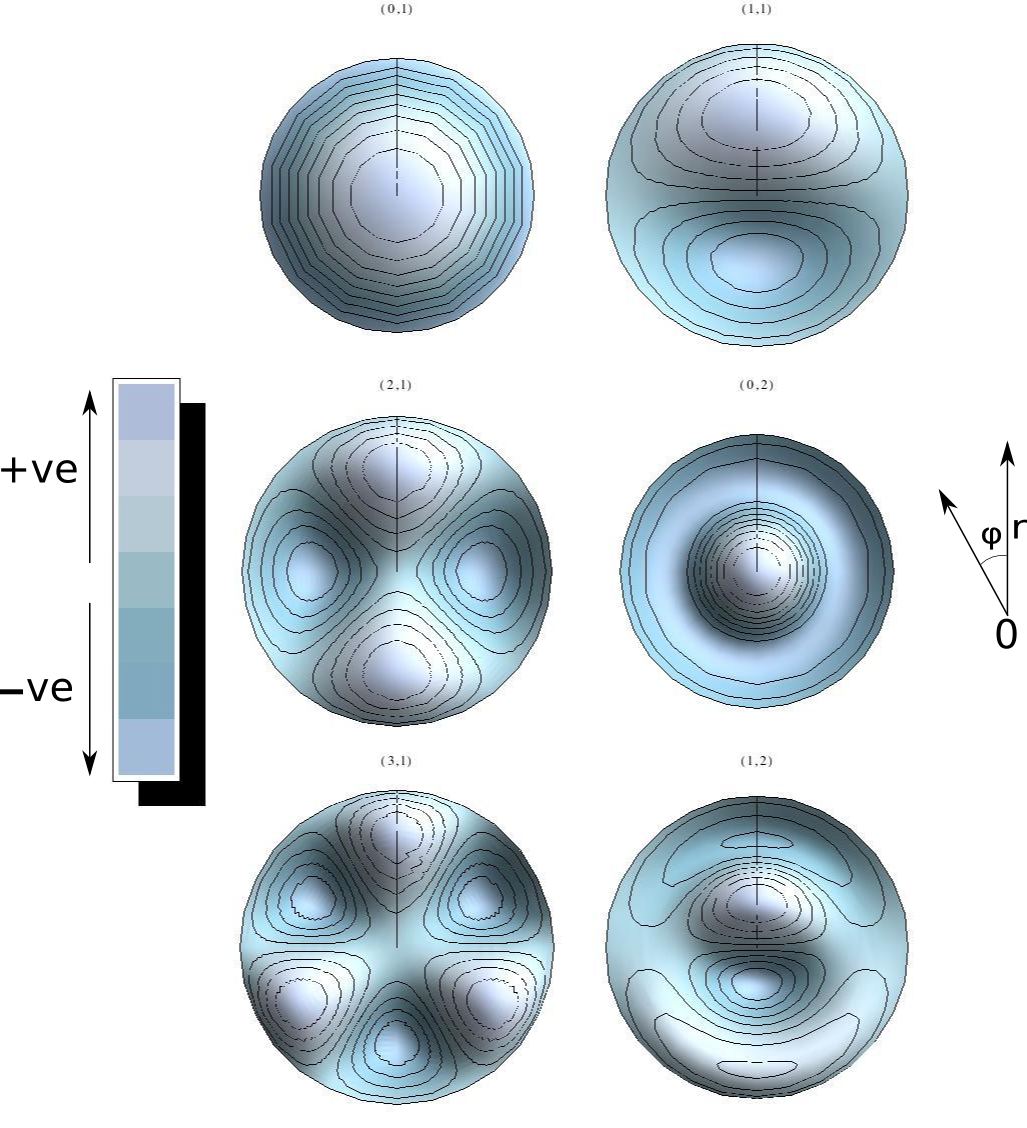
\includegraphics[width=.6\linewidth]{Diagrams/CircularMembraneModes/circular_modes_all.png}
 \caption[Circular membrane eigenmodes]{Eigenmodes of a full circular membrane. The eigenfrequency increases from left to right.}
  \label{circularmembraneeigenmodes}
\end{figure}

We note that unlike in the case of the internal cavity, the free membrane has components
that are both forward- and backward-moving in time. The presence of a driving force, however, will result in simpler expressions. This
will be discussed in more detail in the next chapter where we compare our model with experimental data.

\vspace{\baselineskip}
\noindent\textbf{Damped Membrane}: For a damped membrane, i.e. $\alpha\neq 0$, the spatial part of the above eigenmodes remains the same. The form of the
time-dependent part is given by the solution of the equation,
\begin{equation}\label{dampedtimepart}
 \frac{d^2 h_{mn}(t)}{dt^2}+2\alpha \frac{d h_{mn}(t)}{dt}+\omega_{mn}^2h_{mn}(t)=0.
\end{equation}
Assuming $h_{mn}$ takes the form $e^{j\widetilde{\omega}_{mn}}$ leads to a quadratic equation with solutions,
\begin{align}
 \widetilde{\omega}_{mn}&=j\alpha\pm\omega_{mn}^*\\
 \omega_{mn}^*&=\sqrt{\alpha^2+\omega^2_{mn}}
\end{align}
We require the membrane displacement to remain finite as $t\rightarrow\infty$. We can therefore neglect the $e^{-j\widetilde{\omega}_{mn}}$ terms leading
to,
\begin{equation}\label{circularmembranedampedeigen}
 \widetilde{u}_{mn}(r,\phi;t)=\cos m\phi J_m(\mu_{mn} r)\left[M_{mn}e^{j\omega_{mn}^* t}+N_{mn}e^{-j\omega_{mn}^* t}\right]e^{-\alpha t}
\end{equation}
The general solution is given by a linear combination of the above and the coefficients are determined by initial conditions -- for example,
membrane displacement and velocity at $t=0$.
\subsubsection*{Forced Vibrations}
For a periodically driven membrane, there are two components of the full solution for forced vibrations. The first of these is the steady state solution which
oscillates with the same frequency as the input and does not depend on the initial conditions - $u_{ss}$. The second of these is the transient solution that depends
on the initial conditions but not on the driving pressure - $u_t$. 

\noindent\textbf{Steady State Solution}: The steady state solution is expressed as a linear combination of the spatial part
of the above eigenmodes and is given by,
\begin{equation}\label{membraness1}
 u_{ss}(r,\phi ;t)=\displaystyle\sum^\infty_{m=0}\sum^\infty_{n=1} C_{mn}\cos m\phi J_m(\mu_{mn} r)e^{j\omega t}.
\end{equation}
Substituting this expression in \eqref{membraneequation1} with $\Psi=pe^{j\omega t}$ gives,
\begin{align}
 &\displaystyle\sum^\infty_{m=0}\sum^\infty_{n=1} \Omega_{mn}C_{mn}\cos m\phi J_m(\mu_{mn} r)e^{j\omega t}=pe^{j\omega t}\label{membraness2}\\
 &\text{where,  }\Omega_{mn}=\rho_M d \left[(\omega^2-\omega^2_mn)-2j\alpha\omega\right]\label{omegafirstdef}.
\end{align}
Using the orthogonality of the eigenmodes, the coefficients $C_{mn}$ can be calculated,
\begin{equation}\label{sscoeffs}
 C_{mn}=\frac{p\int dS u_{mn}}{\Omega_{mn}\int dS u^2_{mn}}
\end{equation}
with the integral this time being taken over the circular disk of radius $a_M$.

\vspace{\baselineskip}
\noindent\textbf{Transient Solution}: The transient solution is effectively a solution of the free damped membrane, i.e. a linear 
combination of the eigenmodes given in \eqref{circularmembranedampedeigen}. Therefore,
\begin{equation}\label{membranet1}
 u_t(r,\phi;t)=\displaystyle\sum^\infty_{m=0}\sum^\infty_{n=1}\cos m\phi J_m(\mu_{mn} r)\left[M_{mn}e^{j\omega_{mn}^* t}+N_{mn}e^{-j\omega_{mn}^* t}\right]e^{-\alpha t}.
\end{equation}
The complete solution is given by $u=u_t+u_{ss}$ and the coefficients $M_{mn}$ and $N_{mn}$ are determined by the initial conditions (at $t=0$).

\vspace{\baselineskip}
\textbf{Steady State Approximation}: The damping coefficient $\alpha$ is usually given in terms of the membrane fundamental frequency and a quality factor $Q$ as $\alpha=\omega_{01}/2Q$. For the tympani
we will be concerned with we have $Q\sim 1.2$ which results in damping coefficients that are around $4000s^{-1} $ for the larger lizards and around $8000s^{-1}$ for the smaller ones. 
Due to this and the exponential decay of the transient vibration amplitude, we can safely assume that within a few time-periods the steady-state vibrations dominate the solution of the
forced membrane. For this reason, we will subsequently confine our discussion to only the steady state vibrations of the membrane.
\subsubsection{Sectoral Membrane}
The eigenmodes of the sectoral membrane proceeds from \eqref{membraneeigen} onwards. We now have a new set of boundary conditions in $\phi$.
The extracolumella is modelled as a triangular plate of infinite mass which constrains the membrane displacement to go to zero at $phi=\beta$
and $\phi=2\pi-\beta$. This results in the following set of eigenmodes,
\begin{equation}\label{sectoraleigenmode}
 u_{mn}(r,\phi;t)=\sin \kappa(\phi-\beta) J_\kappa(\mu_{mn} r)\left[M_{mn}e^{j\omega_{mn} t}+N_{mn}e^{-j\omega_{mn} t}\right]
\end{equation}
where $\kappa[m]=\frac{m\pi}{2(\pi-\beta)}$, $m=1,2,3,\ldots$. We see that the $r$ part of the above mode is given by the
order-$\kappa$ Bessel function of the first kind; $\mu_{mn}$ being its $n^{th}$ zero, as before. The solution for the damped
membrane follows in an identical way.
It is apparent from the form of the above modes that, unlike in the case of the circular membrane eigenmodes, these modes
are no longer circularly symmetric. We plot the first few of these modes in \ref{sectoralmembraneeigenmodes}. 
\begin{figure}[ht!]
 \centering
 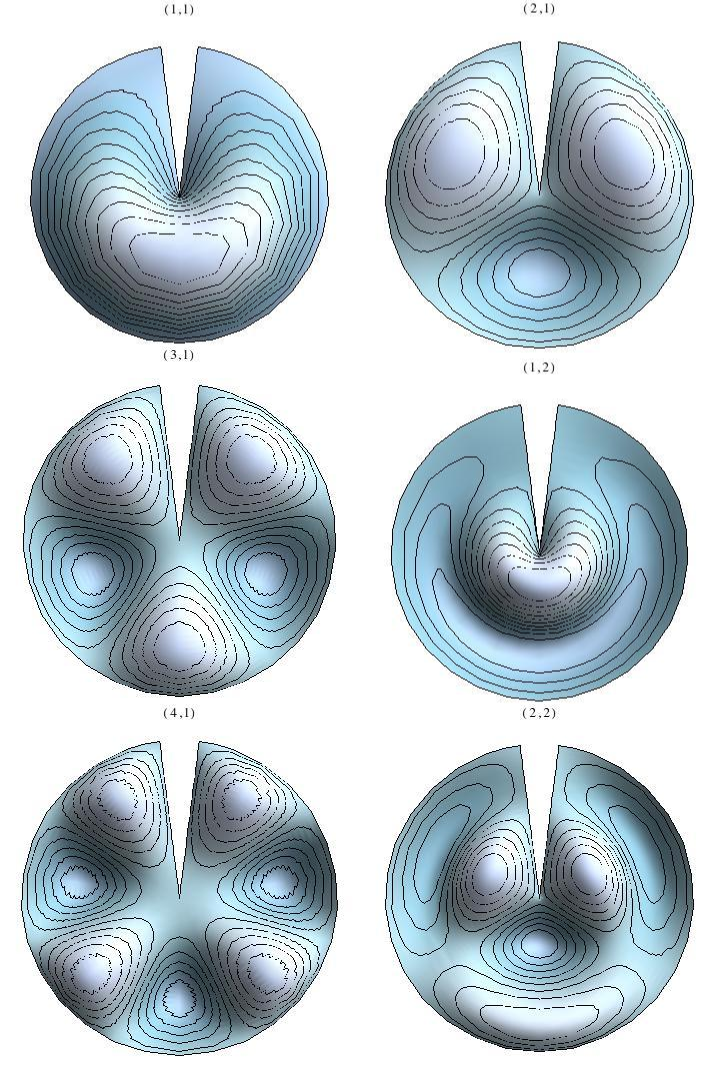
\includegraphics[width=.6\linewidth]{Diagrams/SectorMembraneModes/membrane_modes_all.png}
 \caption[Sectoral membrane eigenmodes]{Eigenmodes of a sectoral membrane with $\beta=\pi/25$. The eigenfrequency increases from left to right.}
  \label{sectoralmembraneeigenmodes}
\end{figure}
The solution for forced membrane vibrations follows in the same way as in the circular membrane case. The vibrations of a sectoral membrane
are discussed in more detail in \cite[p.~87]{fletcheracoustic}. As discussed earlier, the sectoral shape of the membrane has important
physical consequences and captures the complex vibration patterns of a realistic membrane. This will be discussed in the next chapter.
\subsection{Vibration of Coupled Membranes}\label{coupledmembranes}
With our current knowledge, we can move on to the main part of the chapter - the vibration of coupled membranes.
It is convenient to first write down the main equations of the system based on our previously derived expressions.
The vibrations of the membranes is given by,
\begin{equation}\label{coupledmembraneseries}
 u_{0/L}(r,\phi;t)=\displaystyle\sum^{\infty}_{m=0}\sum^{\infty}_{n=1}\Omega_{mn}C^{0/L}_{mn}u_{mn}(r,\phi)e^{j\omega t}=p_{0/L}e^{j\omega t}-p(0/L,r,\phi;t)
\end{equation}
where $0$ and $L$ denote the ipsi- and contra-lateral membranes respectively and the cavity pressure distribution, $p(x,r,\phi;t)$,  is given by \eqref{pressuregeneral1}.
The above equation is only valid on the membrane surface i.e., for $r<a_{tymp}$ and $\beta<\phi<2\pi-\beta$.

As discussed in \ref{pressureboundaryconditions}, the internal cavity pressure satisfies the no-penetration condition at solid boundaries.
This means that at both ends of the cylinder, we equate the velocity profile of air to the velocity profile of the circular surface including
the membrane. This is because the membrane diameter is smaller than the cylinder diameter. As a result, we will have to set the air-particle velocity to zero for $r>a_{tymp}$. 
Since the membrane displacement is
only in the $x$-direction, we only need to calculate the same component of the velocity. Using the relation \eqref{pressurevelocityrelation} we get,
\begin{equation}\label{airvelocity}
v_x(x,r,\phi;t)=-\frac{1}{\rho\omega}\displaystyle\sum^\infty_{q=0}\displaystyle\sum^\infty_{s=0}\zeta_{qs}\left(A_{qs}e^{j\zeta_{qs}x}-B_{qs}e^{-j\zeta_{qs}x}\right)f_{qs}(r,\phi)e^{j\omega t}
\end{equation}
and the exact boundary conditions are given by,
\begin{align}
 j\omega U_{0}&=v_x(0,r,\phi;t)\label{bc1}\\
 j\omega U_{L}&=-v_x(L,r,\phi;t)\label{bc2}
 \end{align}
where we've used the direction conventions described in \ref{description} and made the following definition,
\begin{equation}
 U_{0/L}=\begin{cases}
          u_{0/L}\mbox{, } 0<r<a_{tymp}\mbox{ and } \beta<\phi<2\pi-\beta\\
          0\mbox{, otherwise}
         \end{cases}.
\end{equation}
This in order to ensure that the boundary condition is satisfied over either end of the cylinder and not just over the membrane surface.
\subsubsection{Approximate Boundary Condition}
As previously stated, the exact boundary condition would entail setting the velocity function to be exactly equal to the membrane displacement velocity. At this point, it is important to
note that the internal cavity eigenmodes are \textbf{not} orthogonal to the membrane eigenmodes in general\footnote{This would also be true if we had full circular membranes on either end of the
cylinder. In this case we would have the added simplification that only the circularly symmetric cavity eigenmodes will be activated.}. This means that every membrane eigenmode
couples with every cavity eigenmode and that each of the coefficients $A_{qs}$ and $B_{qs}$ will be given by an infinite linear combination of the coefficients $C^{0/L}_{mn}$. 

The first step in overcoming this problem is to rewrite the left-hand sides of the boundary conditions given in \eqref{bc1} and \eqref{bc2}.
We first expand $U_{0}$ and $U_{L}$ in the orthogonal basis of the functions $f_{qs}$,
\begin{align}
 U_{0/L}(r,\phi;t)&=\displaystyle\sum^\infty_{q=0}\displaystyle\sum^\infty_{s=0} S^{0/L}_{qs}f_{qs}(r,\phi)e^{j\omega t}\\
 \mbox{where, }S^{0/L}_{qs}&=\frac{\int dS U^{0/L}f_{qs}(r,\phi)}{\int dS f^2_{qs}(r,\phi)}\label{approxboundarydef2}
\end{align}

We now have an expansion that approximates the boundary condition with increasing accuracy. After choosing an appropriate cutoff
for the expansion we can substitute this expression in place of $U_{0/L}$ in \eqref{bc1} and \eqref{bc2}. In fact, this cutoff in
the boundary condition expansion results in an identical cutoff in the pressure expansion - a direct result of the orthogonality
of the pressure modes. 

We will now illustrate a solution to the problem by solving the problem with the zeroeth order boundary conditions. 
In the end, it will turn out that for our purposes the zeroeth order, i.e. the $(0,0)$ mode is sufficient as higher modes only have a significant contribution at frequencies
well above the hearing range of geckos. For example, the wavenumber of the $(1,1)$ mode is above $33$kHz for the cylindrical cavity corresponding to the house gecko and 
above $15$kHz for the one corresponding to the Tokay gecko. The parameters used to derive these quantities will be discussed in the next chapter.
We can therefore write the approximate boundary conditions to zeroeth order as,
\begin{align}
   \rho\omega^2S^{0}&=\displaystyle\sum^\infty_{q=0}\displaystyle\sum^\infty_{s=0}j\zeta_{qs}\left(A_{qs}-B_{qs}\right)f_{qs}(r,\phi) \label{bcfinal1}\\
   \rho\omega^2S^{L}&=-\displaystyle\sum^\infty_{q=0}\displaystyle\sum^\infty_{s=0}j\zeta_{qs}\left(A_{qs}e^{j\zeta_{qs}L}-B_{qs}e^{-j\zeta_{qs}L}\right)f_{qs}(r,\phi) \label{bcfinal2}
\end{align}
As shown in Sec. \ref{internalcavity}, the $(0,0)$ mode only varies in the $x$-direciton.
As a result, the left-hand sides of
the above equation are nothing but the average displacement of the membrane surface given by,
\begin{equation}\label{averagemembranedisp}
 S^{0/L}=\frac{\int dS U^{0/L}(r,\phi)}{\pi a^2_{cyl}}.
\end{equation}
We have also omitted the ``$qs$'' subscript from $S^{0/L}$. 
Given the external parameters and boundary conditions, it only depends on time.
We have effectively approximated the surfaces at $0$ and $L$ (including the membranes) by pistons moving with the average velocity of the total surface.

Given these boundary conditions, it is straightforward to calculate the coefficients $A_{qs}$ and $B_{qs}$ in terms of $S_{0/L}$. To do this
we need to make use of the orthogonality relation given in \eqref{besselorthogonality}. We do this by multiplying both sides of \eqref{bcfinal1} and \eqref{bcfinal2}
by $f_{qs}(r,\phi)$ and integrate over the circular surfaces at either end of the cylinder. This results in a system of two linear equations for each pair of $A_{qs}$ 
and $B_{qs}$,
\begin{align}
 &A_{qs}-B_{qs} = K_{qs}\rho\omega^2S^{0}\\
 &A_{qs}e^{j\zeta_{qs}L}-B_{qs}e^{-j\zeta_{qs}L} = - K_{qs}\rho\omega^2S^{L}\\
 \mbox{where,}\ &K_{qs} = \frac{\int dS f_{qs}(r,\phi)}{j\zeta_{qs}\int dS f^2_{qs}(r,\phi)}\nonumber
\end{align}
We now make use of the property of the pressure modes that $f_{qs}(r,\phi)$ integrates to $0$ unless $q=0$ and $s=0$. 
For $q=0$ this is a consequence of the Bessel functions integrating to zero while for $q\geq 1$ this is due to 
the more obvious fact that the integral of the cosine function from $0\mbox{ to }2\pi$ is zero. As a result we have $A_{qs}=B_{qs}=0$ for all
modes except the $(0,0)$ mode. In other words, the zeroeth-order boundary condition only supports plane wave
modes inside the cavity. We will subsequently omit the subscripts ``$00$'' for these coefficients.
From the above linear equations, they are given in terms of the total membrane displacement as,
\begin{equation}\label{finalpressurecoefficients}
 A=\frac{\rho\omega^2}{2 k\sin kL}\left(S^0e^{-jkL}+S^L\right),\qquad  B=\frac{\rho\omega^2}{2 k\sin kL}\left(S^0e^{jkL}+S^L\right)
\end{equation}
we have also directly substituted $\zeta_{00}=k$ and simplified the expression for $K_{00}$ in the above expressions. These
coefficients can now be substituted in place of the pressure in the right-hand side of the equation \eqref{coupledmembraneseries}
giving us,
\begin{align}
 &\displaystyle\sum^\infty_{m=0}\displaystyle\sum^\infty_{n=1}\Omega_{mn}C^{0}_{mn}u_{mn}(r,\phi)=p_{0}-\frac{\rho\omega^2}{k}\left(S^0\cot kL+S^L\csc kL\right)\\
 &\displaystyle\sum^\infty_{m=0}\displaystyle\sum^\infty_{n=1}\Omega_{mn}C^{L}_{mn}u_{mn}(r,\phi)=p_{L}-\frac{\rho\omega^2}{k}\left(S^0\csc kL+S^L\cot kL\right)
\end{align}
where we have cancelled out the time component on both sides of the equations. Note that the right-hand sides of the above two equations
are independent of the spatial $(r,\phi)$ coordinates.

In order to simplify the above coupled system of equations, the next step will be to take their sum and difference to obtain a new set of 
variables that are solutions of a pair of decoupled equations. After some algebraic manipulation, we therefore have
\begin{align}
 &\displaystyle\sum^\infty_{m=0}\displaystyle\sum^\infty_{n=1}\Omega_{mn}C^{+}_{mn}u_{mn}(r,\phi)=p_{+}-\frac{\rho\omega^2}{k}S^+\cot \frac{kL}{2}\\
 &\displaystyle\sum^\infty_{m=0}\displaystyle\sum^\infty_{n=1}\Omega_{mn}C^{-}_{mn}u_{mn}(r,\phi)=p_{-}-\frac{\rho\omega^2}{k}S^-\tan \frac{kL}{2}
\end{align}
where, $C_{mn}^+=C_{mn}^L+C_{mn}^0$ and $C_{mn}^-=C_{mn}^L-C_{mn}^0$. The $S^{+/-}$ and $p_{+/-}$ terms are defined similarly.
Now, analogous to the calculation of the coefficients for the steady state vibration in \eqref{membraness2} and \eqref{sscoeffs}, we can determine
the coefficients of the sum and difference vibrations in terms of the pressure and total membrane displacements. This gives us,
\begin{align}
 C^{+}_{mn}&=\left[p_{+}-\frac{\rho\omega^2}{k}S^+\cot \frac{kL}{2}\right]K_{mn}\label{pluscoeffdef}\\
 C^{-}_{mn}&=\left[p_{-}-\frac{\rho\omega^2}{k}S^-\tan \frac{kL}{2}\right]K_{mn}\label{minuscoeffdef}\\
 \mbox{where, }K_{mn}&=\frac{\int dS u_{mn}}{\Omega_{mn}\int dS u^2_{mn}}\nonumber
\end{align}
The next step will be to multiply both sides of \eqref{pluscoeffdef} and \eqref{minuscoeffdef} with the integral $\int dS u_{mn}$, 
divide by $\pi a^2_{cyl}$ (the integral of $f^2_{00}$ as it appears in the denominator in \eqref{approxboundarydef2}) and
sum over $m\mbox{ and }n$ . It is clear that the left hand sides become equal to $S^{+/-}$; this allows us to give exact expressions
for the total membrane displacements.
\begin{equation}
 S^{+}=\frac{p_L+p_0}{\Lambda+\Gamma_+}\qquad S^{-}=\frac{p_L-p_0}{\Lambda+\Gamma_-}
\end{equation}
where we've defined the following quantities,
\begin{align}
 \Gamma_+ = \frac{\rho\omega^2}{k}\cot \frac{kL}{2},\qquad \Gamma_-= \frac{\rho\omega^2}{k}\tan \frac{kL}{2}\nonumber
,\qquad\frac{1}{\Lambda}=\frac{1}{\pi a^2_{cyl}}\displaystyle\sum^\infty_{m=0}\displaystyle\sum^\infty_{n=1}\frac{\left(\int dS u_{mn}\right)^2}{\Omega_{mn}\int dS u^2_{mn}}\nonumber
\end{align}
We can finally write the membrane displacement as a function of the pressure inputs in the form
\begin{align}
 u_0(r,\phi;t)&=G_{ipsi}(r,\phi)p_0+G_{contra}(r,\phi)p_L\label{ipsimembranefull}\\
 u_L(r,\phi;t)&=G_{contra}(r,\phi)p_0+G_{ipsi}(r,\phi)p_L\label{contramembranefull}
\end{align}
with the ipsilateral filter,
\begin{equation}
 G_{ipsi}=\left(\frac{1}{\Lambda+\Gamma_+}+\frac{1}{\Lambda+\Gamma_-}\right)\displaystyle\sum^\infty_{n=1}\frac{\Lambda K_{mn}}{2}u_{mn}(r,\phi;t)
\end{equation}
and the contralateral filter,
\begin{equation}
 G_{contra}=\left(\frac{1}{\Lambda+\Gamma_+}-\frac{1}{\Lambda+\Gamma_-}\right)\displaystyle\sum^\infty_{n=1}\frac{\Lambda K_{mn}}{2}u_{mn}(r,\phi;t)
\end{equation}
The total membrane displacement can also be expressed as a function of $p_0$ and $p_L$ simply by integrating both sides of \eqref{ipsimembranefull}
and \eqref{contramembranefull} giving us a new set of ipsi- and contralateral filters
\begin{align}
 G^s_{ipsi}&=\left(\frac{1}{\Lambda+\Gamma_+}+\frac{1}{\Lambda+\Gamma_-}\right)/2\\
 G^s_{contra}&=\left(\frac{1}{\Lambda+\Gamma_+}-\frac{1}{\Lambda+\Gamma_-}\right)/2
\end{align}
The ipsilateral filter effectively gives us the response of the ipsilateral membrane when the contralateral membrane
is blocked. Similarly, the contralateral filter gives us its response when there is no ipsilateral stimulus. These filters
will play an important role in the evaluation of the model in the next chapter.

\subsection{Circuit Model}
Before we conclude this chapter, we will discuss the previous methods used to model ears coupled through
an air cavity. This method was used by Christensen-Dalsgaard and Manley in \cite{dalsgaardmanley1} and \cite{dalsgaardmanley2}
and was based on methods presented in \cite{fletcheracoustic}. The method treats the problem through the analogy of electrical circuits
and deals with low-frequency and high-frequency regimes separately.

In these models, the sound inputs are treated as voltage sources and the system is broken down into components, e.g.	 membranes,
cavities, apertures which are modelled as lumped elements. Their impedance values depend on the geometry and material properties and in general
 can be resistive and reactive. The ``current'' is given by something called the ``acoustic flow'' which has the dimensions of
volume per unit time. In the previous analysis, this is given by $j\omega\pi a^2_{cyl}S^{0/L}$. 

The low frequency circuit analog for the ICE model is illustrated in Fig. \ref{lowfreqcircuit}. The impedances are calculated
using the following formulae,
\begin{align}
 &R_T=\frac{\omega_TL_T}{Q},\qquad L_T=\frac{\rho_Md}{\pi a_{tymp}^2},\qquad C_T=\frac{1}{\omega^2_TL_T}\\
 &R_V=0,\qquad L_V=0,\qquad C_V=\frac{V_0}{\rho c^2}
\end{align}
where $R,\ L\mbox{ and }C$ are the resistance, impedance and capacitance of the quantities respectively with the total impedance
given by $Z=R+j\omega L+1/j\omega C$. $\omega_T$ is the first eigenfrequency of the membrane.
\begin{figure}[ht!]
 \centering
 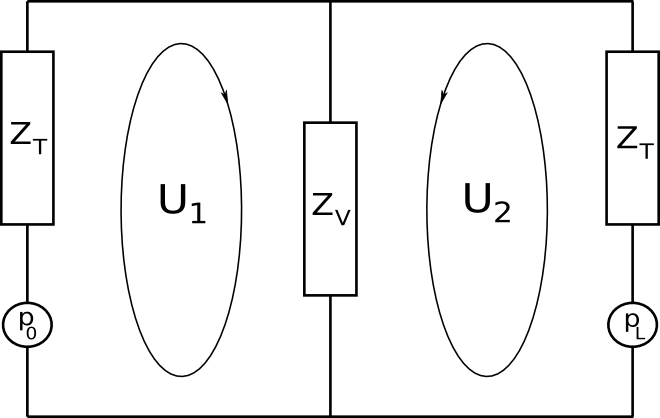
\includegraphics[width=.5\linewidth]{Diagrams/lowfreqcircuit.png}
 \caption[Low frequency circuit analog]{Low frequency circuit analog for the ICE-Model. The membrane impedences are denoted by $Z_T$ and the impedance of 
 the internal cavity is denoted by $Z_V$. The acoustic flows are given by $U_1\mbox{ and }U_2$.}
  \label{lowfreqcircuit}
\end{figure}
It should immediately be apparent that the cavity impedance only depends on its volume. This is a result of the assumption 
that the air inside the cavity behaves like an adiabatic gas. The adiabatic equation of state can then be used
to determine the instantaneous pressure from the instantaneous volume change due to the membrane
motion which, after linearization, results in a uniform pressure inside the cavity. In addition, the membrane impedance $Z_T$ only includes the
effect of the first eigenmode. Also, $Z_T$ includes the effect of the transducer which, in our case, is the extracolumella. Upon solving the circuit equations, the acoustic flows are calculated to be,
\begin{equation}
 U_1=\frac{p_0(Z_T+Z_V)-p_LZ_V}{Z_T(Z_T+2Z_V)},\qquad U_2=\frac{p_L(Z_T+Z_V)-p_0Z_V}{Z_T(Z_T+2Z_V)}.
\end{equation}
At first glance the above results look very similar to total membrane displacements shown in \eqref{ipsimembranefull} and \eqref{contramembranefull}.
In fact, we can find the equivalent impedances from our analysis by comparing $U_0$ and $U_L$ with the above results,
\begin{equation}
 Z^{eq}_T=\frac{1}{j\omega\pi a^2_{cyl}}(\Lambda+\Gamma_-),\qquad Z^{eq}_V=\frac{1}{2j\omega\pi a^2_{cyl}}(\Gamma_+-\Gamma_-)
\end{equation}
We immediately see that in the equivalent membrane impedance there is a correction, $\Gamma^+$ which is a contribution of the cavity whereas in 
the circuit model, the membrane impedance is determined independent of the cavity. Moreover, the equivalent standalone membrane impedance, $\Lambda$,
includes the influence of the higher modes. The equivalent cavity impedance becomes equal to $Z_V$ at zero frequency and goes to infinity at the
resonance frequencies of the cylinder, i.e at $\omega=n\pi c/L,\ n=0,1,2\ldots$
% At high frequencies, i.e. when the wavelength of the input becomes comparable with the dimensions of the system, the description of the
% membrane does not change but the cavity impedance has a frequency dependent addition instead modelled as a two-port network. 
% 
% \begin{figure}[ht!]
%  \centering
%  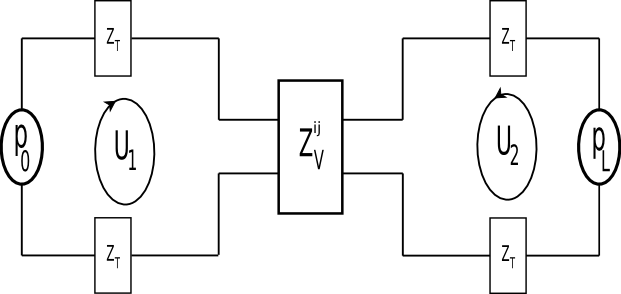
\includegraphics[width=.75\linewidth]{Diagrams/highfreqcircuit.png}
%  \caption[High frequency circuit analog]{High frequency circuit analog for the ICE-Model.}
%   \label{highfreqcircuit}
% \end{figure}
\vspace{\baselineskip}

\noindent We conclude this chapter by briefly stating the advantages of our method in comparison to the lumped element method - 
\begin{itemize}
 \item In terms of the membrane motion - we are able to account for the effect of asymetrically loaded extracolumella and are able to describe the membrane motion is spatial detail.
 \item At low frequencies our model is consistent with the uniform pressure assumption but the nonuniformity steadily increases with frequency.
  We therefore have a single model that can describe both high- and low-frequency behaviour instead of treating the two regimes separately.
\end{itemize}

